% Promoted from L18; H9 gradient geometry retained. One website/handout source.
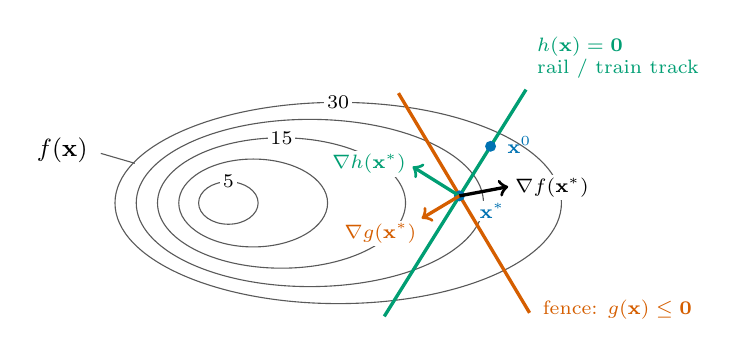
\begin{tikzpicture}[scale=0.90,every node/.style={font=\scriptsize}]
\definecolor{cifenceorange}{HTML}{D55E00}
\definecolor{cifenceblue}{HTML}{0072B2}
\definecolor{cifencegreen}{HTML}{009E73}
  \foreach \cx/\rx/\ry in {1.00/0.42/0.30, 1.35/1.05/0.62, 1.75/1.75/0.92,
                           2.15/2.45/1.18, 2.55/3.15/1.42}
    \draw[black!65] (\cx,1.8) ellipse ({\rx} and {\ry});
  \node[fill=white,inner sep=1pt] at (1.00,2.10) {5};
  \node[fill=white,inner sep=1pt] at (1.75,2.72) {15};
  \node[fill=white,inner sep=1pt] at (2.55,3.22) {30};
  \node[anchor=east,font=\small] at (-0.85,2.55) {$f(\mathbf{x})$};
  \draw[black!65] (-0.80,2.50) -- (-0.32,2.36);
  % fence
  \draw[very thick,cifenceorange] (3.40,3.35) -- (5.25,0.25);
  \node[cifenceorange,anchor=west] at (5.30,0.30) {fence: $g(\mathbf{x}) \le \mathbf{0}$};
  % rail
  \draw[very thick,cifencegreen] (3.20,0.20) -- (5.20,3.40);
  \node[cifencegreen,anchor=south west,align=left] at (5.22,3.42)
    {$h(\mathbf{x})=\mathbf{0}$\\rail / train track};
  % ball starts high on the rail and slides down it to x*
  \fill[cifenceblue] (4.70,2.60) circle (2.2pt);
  \node[cifenceblue,anchor=west] at (4.80,2.62) {$\mathbf{x}^0$};
  \fill[cifenceblue] (4.26,1.90) circle (2.2pt);
  % Label placed down-and-right: the only direction at x* free of an arrow,
  % the fence and the rail.
  \node[cifenceblue,anchor=north west,fill=white,inner sep=1pt] at (4.50,1.84)
    {$\mathbf{x}^*$};
  % Three GRADIENT arrows at x*, each normal to its own level set and coloured
  % to match it: grad h green along the rail normal, grad g red along the fence
  % normal (pointing to the infeasible side), grad f black along the contour
  % normal. Directions computed -- see the geometry note below.
  \draw[->,very thick,cifencegreen] (4.26,1.90) -- (3.599,2.313);
  \node[cifencegreen,anchor=east,fill=white,inner sep=1pt] at (3.55,2.35)
    {$\nabla h(\mathbf{x}^*)$};
  \draw[->,very thick,cifenceorange] (4.26,1.90) -- (3.728,1.582);
  \node[cifenceorange,anchor=north east,fill=white,inner sep=1pt] at (3.70,1.56)
    {$\nabla g(\mathbf{x}^*)$};
  \draw[->,very thick] (4.26,1.90) -- (4.948,2.030);
  \node[anchor=west,fill=white,inner sep=1pt] at (5.00,2.02)
    {$\nabla f(\mathbf{x}^*)$};
\end{tikzpicture}
